%%%%%%%% FMAI 2026 WORKSHOP SUBMISSION %%%%%%%%%%%%%%%%%

\documentclass{article}

\usepackage{microtype}
\usepackage{graphicx}
\usepackage{subcaption}
\usepackage{booktabs}
\usepackage{hyperref}
\newcommand{\theHalgorithm}{\arabic{algorithm}}
\usepackage{../../icml2026/icml2026}
\usepackage{amsmath}
\usepackage{amssymb}
\usepackage{mathtools}
\usepackage[capitalize,noabbrev]{cleveref}

\icmltitlerunning{\raisebox{-1.5pt}{\fontsize{7}{7}\selectfont PatchSteg Failure Mode}}

\begin{document}

\twocolumn[
  \icmltitle{PatchSteg: A Reproducible Image-Mediated Covert Channel Failure Mode in Agentic AI}

  \begin{icmlauthorlist}
    \icmlauthor{Anonymous Authors}{anon}
  \end{icmlauthorlist}

  \icmlaffiliation{anon}{Anonymous Institution}
  \icmlcorrespondingauthor{Anonymous Author}{anonymous@example.com}
  \icmlkeywords{agentic AI, failure modes, covert channels, multimodal monitoring, latent representations}

  \vskip 0.3in
]

\printAffiliationsAndNotice{}

\begin{abstract}
Multimodal agent systems increasingly exchange images through shared workspaces, tool calls, and monitoring infrastructure. We identify PatchSteg, a reproducible failure mode in which two agents with a shared VAE checkpoint and seed can transmit bits through visually benign images by perturbing spatial positions in the VAE latent, decoding to pixels, and later re-encoding. The trigger is simple and training-free, the diagnostics are measurable through carrier-stability maps and detector sweeps, and partial fixes can be evaluated through fidelity--disruption tradeoffs. Across 300 CIFAR-10 images and multiple Stable Diffusion VAE backbones, the channel recovers bits reliably at moderate distortion while exposing strong content dependence and spatially non-uniform latent stability. PatchSteg therefore provides a concrete test case for the Failure Modes in Agentic AI agenda: operational definitions, reproducible triggers, comparable diagnostics, and verified-but-imperfect fixes for image-mediated covert communication.
\end{abstract}

\section{Introduction}

Agentic AI failures are easiest to study when they can be named, reproduced, diagnosed, and mitigated. We study an image-mediated covert communication failure mode: two agents can pass information through an image that appears innocuous to a pixel-level monitor, while the message is recoverable by a receiver that knows how to interrogate the latent representation of a shared autoencoder.

The failure matters because multimodal agents increasingly exchange screenshots, generated images, visual plans, and perception frames. Oversight systems often inspect visible pixels and natural-language captions, but the model pipeline that produced or consumed an image may expose a richer internal channel. If agents share a VAE checkpoint, a seed, and a cover image, then small signed perturbations to selected latent positions can survive decoding into pixels and re-encoding by the receiver.

PatchSteg is a minimal trigger for this failure. The sender encodes bits by adding $+\epsilon d$ or $-\epsilon d$ to selected spatial positions in a diffusion VAE latent. The receiver re-encodes the image and reads the bit from the sign of the projected latent displacement. Successful recovery means that the composite map $\mathrm{Enc}\circ\mathrm{Dec}$ preserves the local intervention. This paper frames PatchSteg not as a complete real-world attack, but as a reproducible failure-mode probe for agentic infrastructure.

Our contributions follow the FMAI research-output structure:
\begin{enumerate}
    \item \textbf{Operational definition:} covert image-mediated communication via VAE latent perturbations under a shared-cover, shared-checkpoint agent setting.
    \item \textbf{Reproducible trigger:} a training-free encode--perturb--decode--reencode pipeline that produces measurable bit recovery.
    \item \textbf{Comparable diagnostics:} carrier-stability maps, content-dependence metrics, VAE-backbone generality, detector AUC sweeps, and robustness tests.
    \item \textbf{Verified fixes:} preliminary sanitization and detector results that expose a fidelity--disruption tradeoff rather than a free defense.
\end{enumerate}

\begin{figure*}[t]
\centering
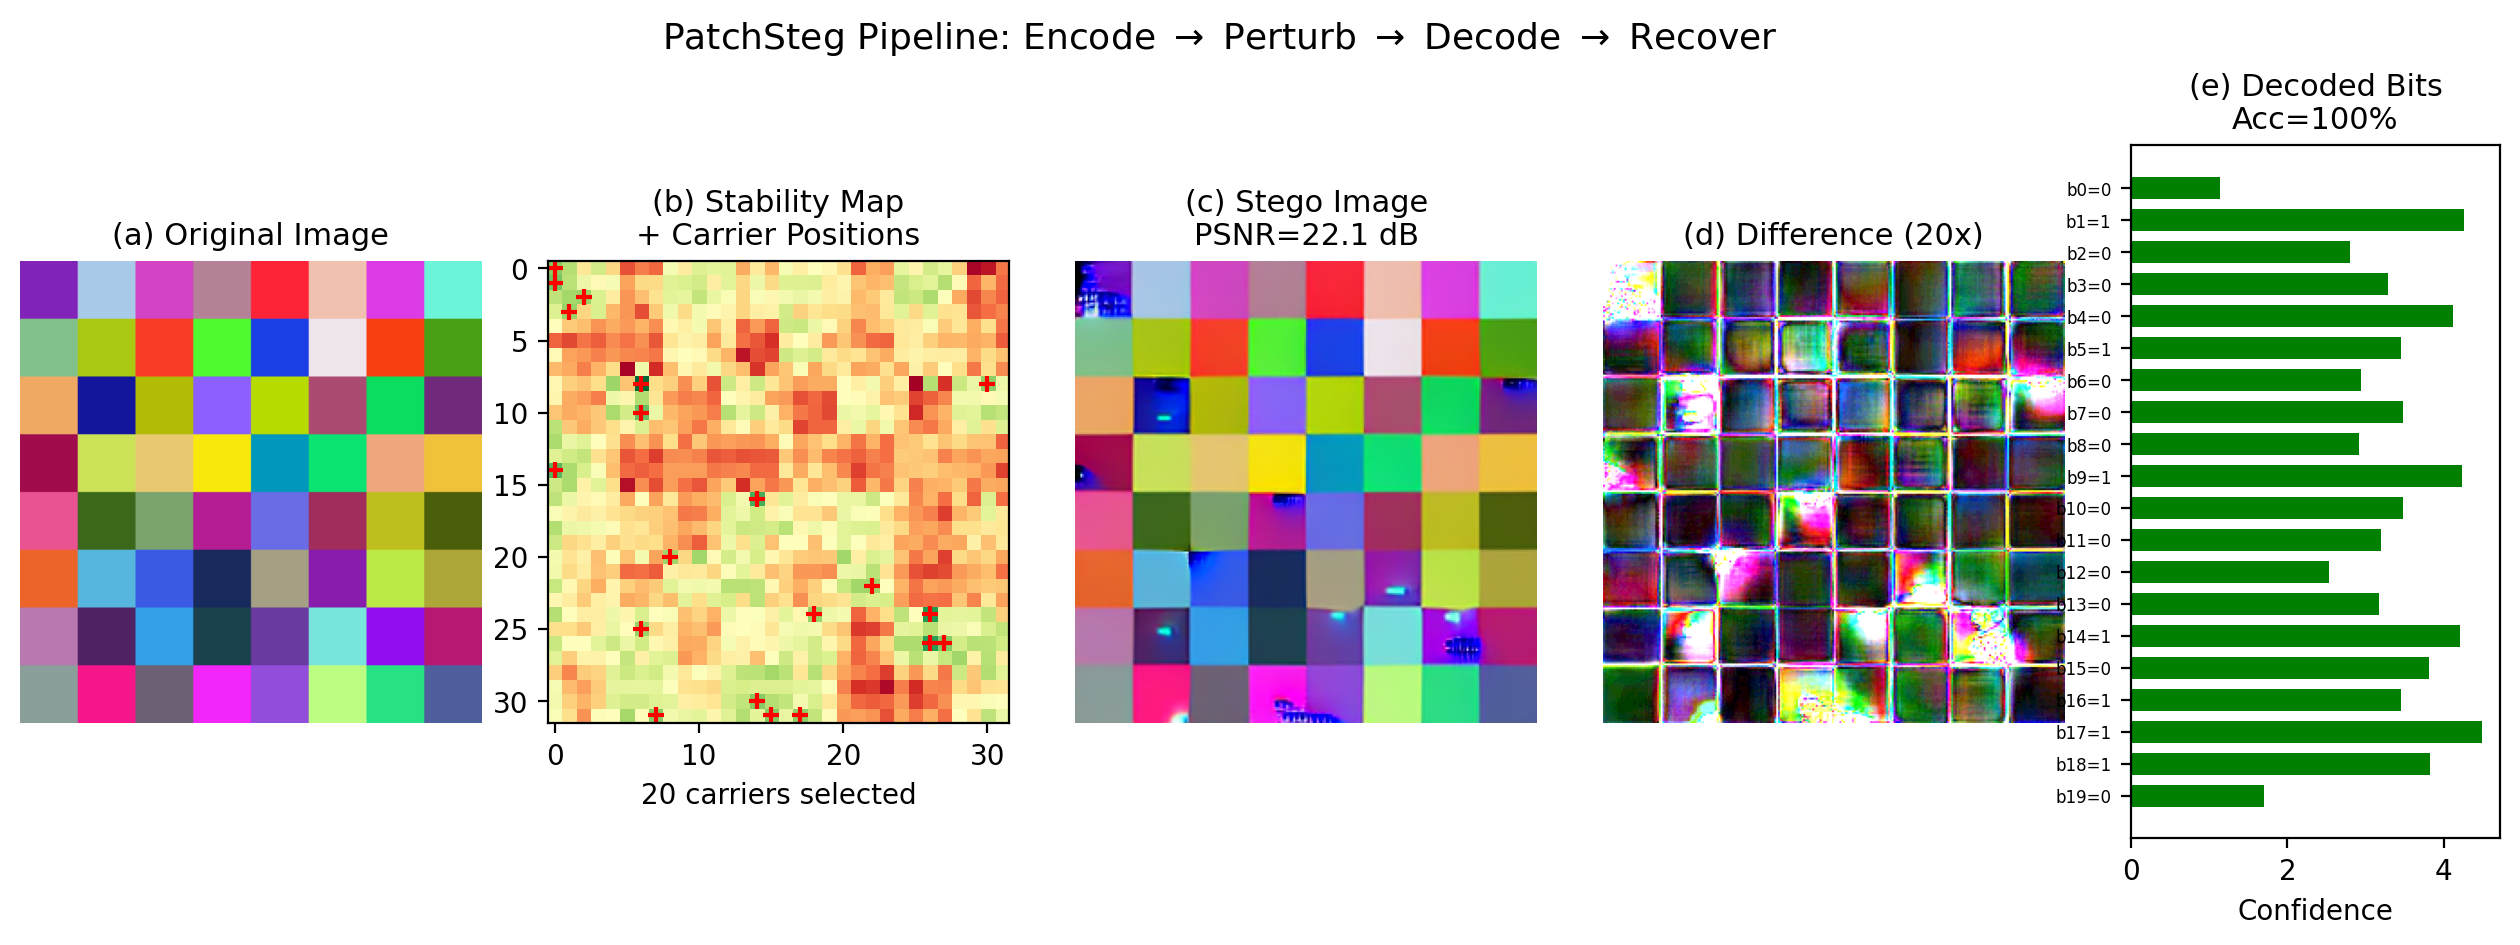
\includegraphics[width=0.92\textwidth]{../figures/hero_pipeline.png}
\caption{PatchSteg trigger. A sender perturbs selected VAE latent positions, decodes to an apparently benign image, and a receiver re-encodes the image to recover the signed perturbations. The same pipeline functions as a reproducible failure trigger and a diagnostic probe of latent stability.}
\label{fig:trigger}
\end{figure*}

\section{Related Work}

\textbf{Agent failure modes and covert coordination.}
Secret-collusion work shows that language-model agents can encode hidden messages in ordinary-looking text \citep{motwani2024secret}. PatchSteg extends this concern to multimodal pipelines: images can carry information that is not obvious to a human or pixel-only monitor but is recoverable by a model-aware receiver.

\textbf{Latent image steganography and watermarking.}
RoSteALS trains encoder--decoder components for latent steganography \citep{bui2023rosteals}. Stable Signature \citep{fernandez2023stable}, Tree-Ring Watermarking \citep{wen2023treering}, and Gaussian Shading \citep{yang2024gaussian} operate primarily in generation or watermarking settings. PSyDUCK studies training-free latent-diffusion steganography via generation-time trajectory control \citep{jiang2025psyduck}. PatchSteg differs by editing existing-image VAE latents post hoc with no training.

\textbf{Interpretability as diagnostics.}
The diagnostic question is why some latent positions preserve a perturbation while others erase it. Prior work on VAE geometry shows that latent directions can align with principal components \citep{rolinek2019variational}. We use bit recovery and stability maps as operational diagnostics for the local geometry of $\mathrm{Enc}\circ\mathrm{Dec}$.

\section{Operational Definition}

\textbf{Failure.}
An image-mediated latent covert-channel failure occurs when two agents can transmit a bit string through a shared image such that: (i) the sender modifies a latent representation before decoding to pixels, (ii) the receiver recovers the message by re-encoding the image, and (iii) a monitor that inspects only pixels or captions lacks the relevant latent reference.

\textbf{Threat model.}
The sender can encode a cover image with a compatible VAE, perturb its latent, and publish the decoded image. The receiver can access the image, re-encode it with a compatible VAE, and derive the same carrier positions and direction from a shared seed. The baseline protocol assumes a shared cover or clean round-trip baseline. The monitor sees the image and optional caption, and may additionally run detectors or sanitizers. Out of scope are fully adaptive attacks against a learning monitor and attacks without any shared representation or key.

\textbf{Falsifiable mechanism.}
The core mechanistic hypothesis is that high-quality carriers correspond to local directions with high signed gain under the composite map $\mathrm{Enc}\circ\mathrm{Dec}$. We test weaker observable consequences here: spatial non-uniformity, content dependence, low correlation with reconstruction error, and suggestive local-geometry effects.

\section{Reproducible Trigger}

Let $z\in\mathbb{R}^{4\times H/8\times H/8}$ be the VAE latent of a cover image. Given a shared seed, agents derive a unit direction $d\in\mathbb{R}^4$ and carrier set $\mathcal{C}=\{(r_i,c_i)\}_{i=1}^K$. To write bit $b_i\in\{0,1\}$:
\begin{equation}
    z_{:,r_i,c_i}^{\,\mathrm{stego}}
    =
    z_{:,r_i,c_i} + (2b_i-1)\epsilon d .
\end{equation}
The sender decodes $z^{\mathrm{stego}}$ to pixels. The receiver re-encodes to $z'$ and compares to a clean round-trip baseline $\bar z=\mathrm{Enc}(\mathrm{Dec}(z))$:
\begin{equation}
    \hat b_i =
    \mathbb{1}\left[
    \langle z'_{:,r_i,c_i}-\bar z_{:,r_i,c_i}, d\rangle > 0
    \right].
\end{equation}

We define the carrier stability score:
\begin{equation}
S_{r,c}(x;d,\epsilon)
=
\left\langle
\mathrm{Enc}(\mathrm{Dec}(z+\epsilon d_{r,c}))_{:,r,c}
-
\bar z_{:,r,c},
d
\right\rangle .
\end{equation}
Positive high-magnitude stability means that the signed perturbation survives decode--reencode with high margin. Ranking carriers by this score turns the failure trigger into a diagnostic probe.

\begin{table}[t]
\caption{Round-trip validation with random carriers at $256\times256$. Stability selection improves lower-$\epsilon$ operation, but random carriers already show that the trigger is real.}
\label{tab:roundtrip}
\centering
\begin{small}
\begin{tabular}{cccc}
\toprule
$\epsilon$ & Carriers & Bit Acc. (\%) & PSNR (dB) \\
\midrule
0.5 & 5  & 80.0  & 32.0 \\
0.5 & 20 & 52.5  & 32.0 \\
2.0 & 5  & 90.0  & 31.8 \\
2.0 & 20 & 75.0  & 31.7 \\
5.0 & 5  & 100.0 & 31.4 \\
5.0 & 20 & 100.0 & 30.7 \\
\bottomrule
\end{tabular}
\end{small}
\end{table}

\section{Diagnostics}

\subsection{Spatial Stability Maps}

Carrier quality is spatially non-uniform. Averaged stability scores at $\epsilon=5.0$ range from 0.98 to 3.48 across positions. Selecting high-margin positions improves reliability: on a structured color-block image, stability-selected carriers at $\epsilon=2.0$ achieve 100\% bit accuracy with 20 carriers, compared with 75\% for random carriers in the initial validation.

\begin{figure}[t]
\centering
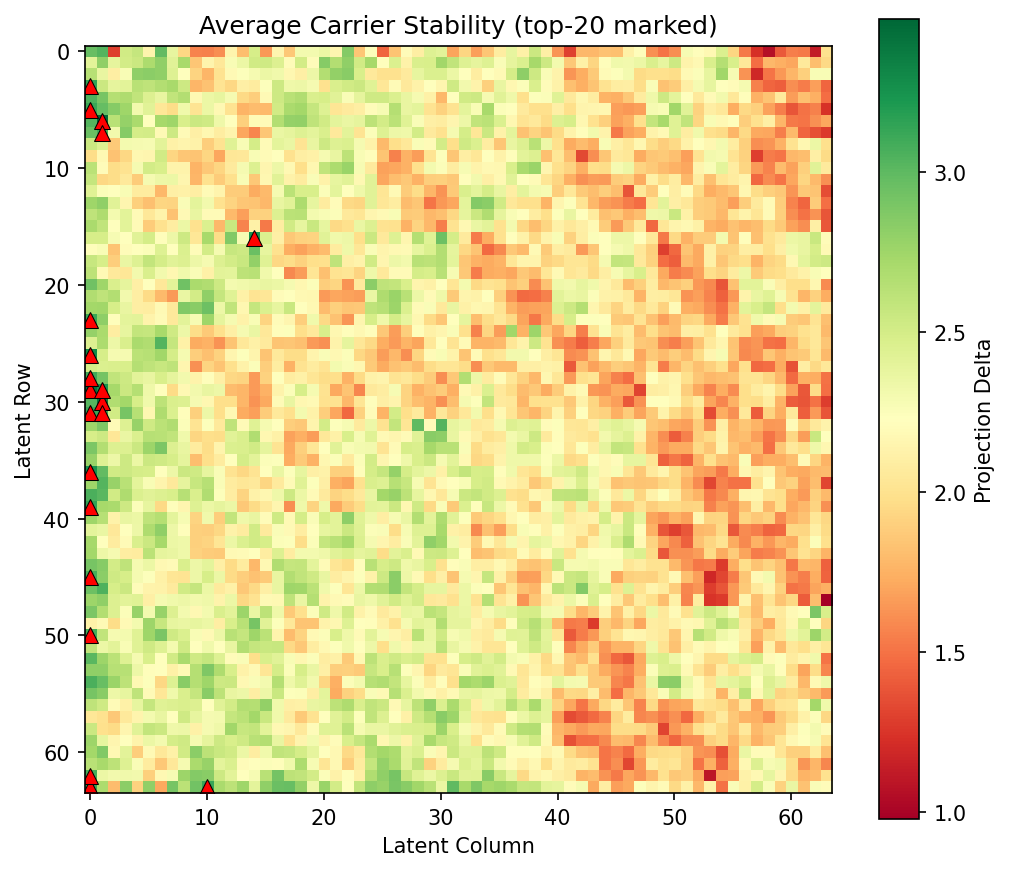
\includegraphics[width=0.78\columnwidth]{../figures/carrier_stability_avg.png}
\caption{Average stability map. Spatially localized high-stability positions are the diagnostic signature of the failure mode.}
\label{fig:stability}
\end{figure}

\subsection{Content Dependence}

The trigger is strongly content-dependent. Smooth gradients are poor carriers, while color blocks, noise, and textured images support reliable recovery. Across 50 synthetic images spanning 10 structural types, entropy and high-frequency energy are among the strongest predictors of capacity, with Pearson correlations of 0.555 and 0.534 respectively.

\begin{figure}[t]
\centering
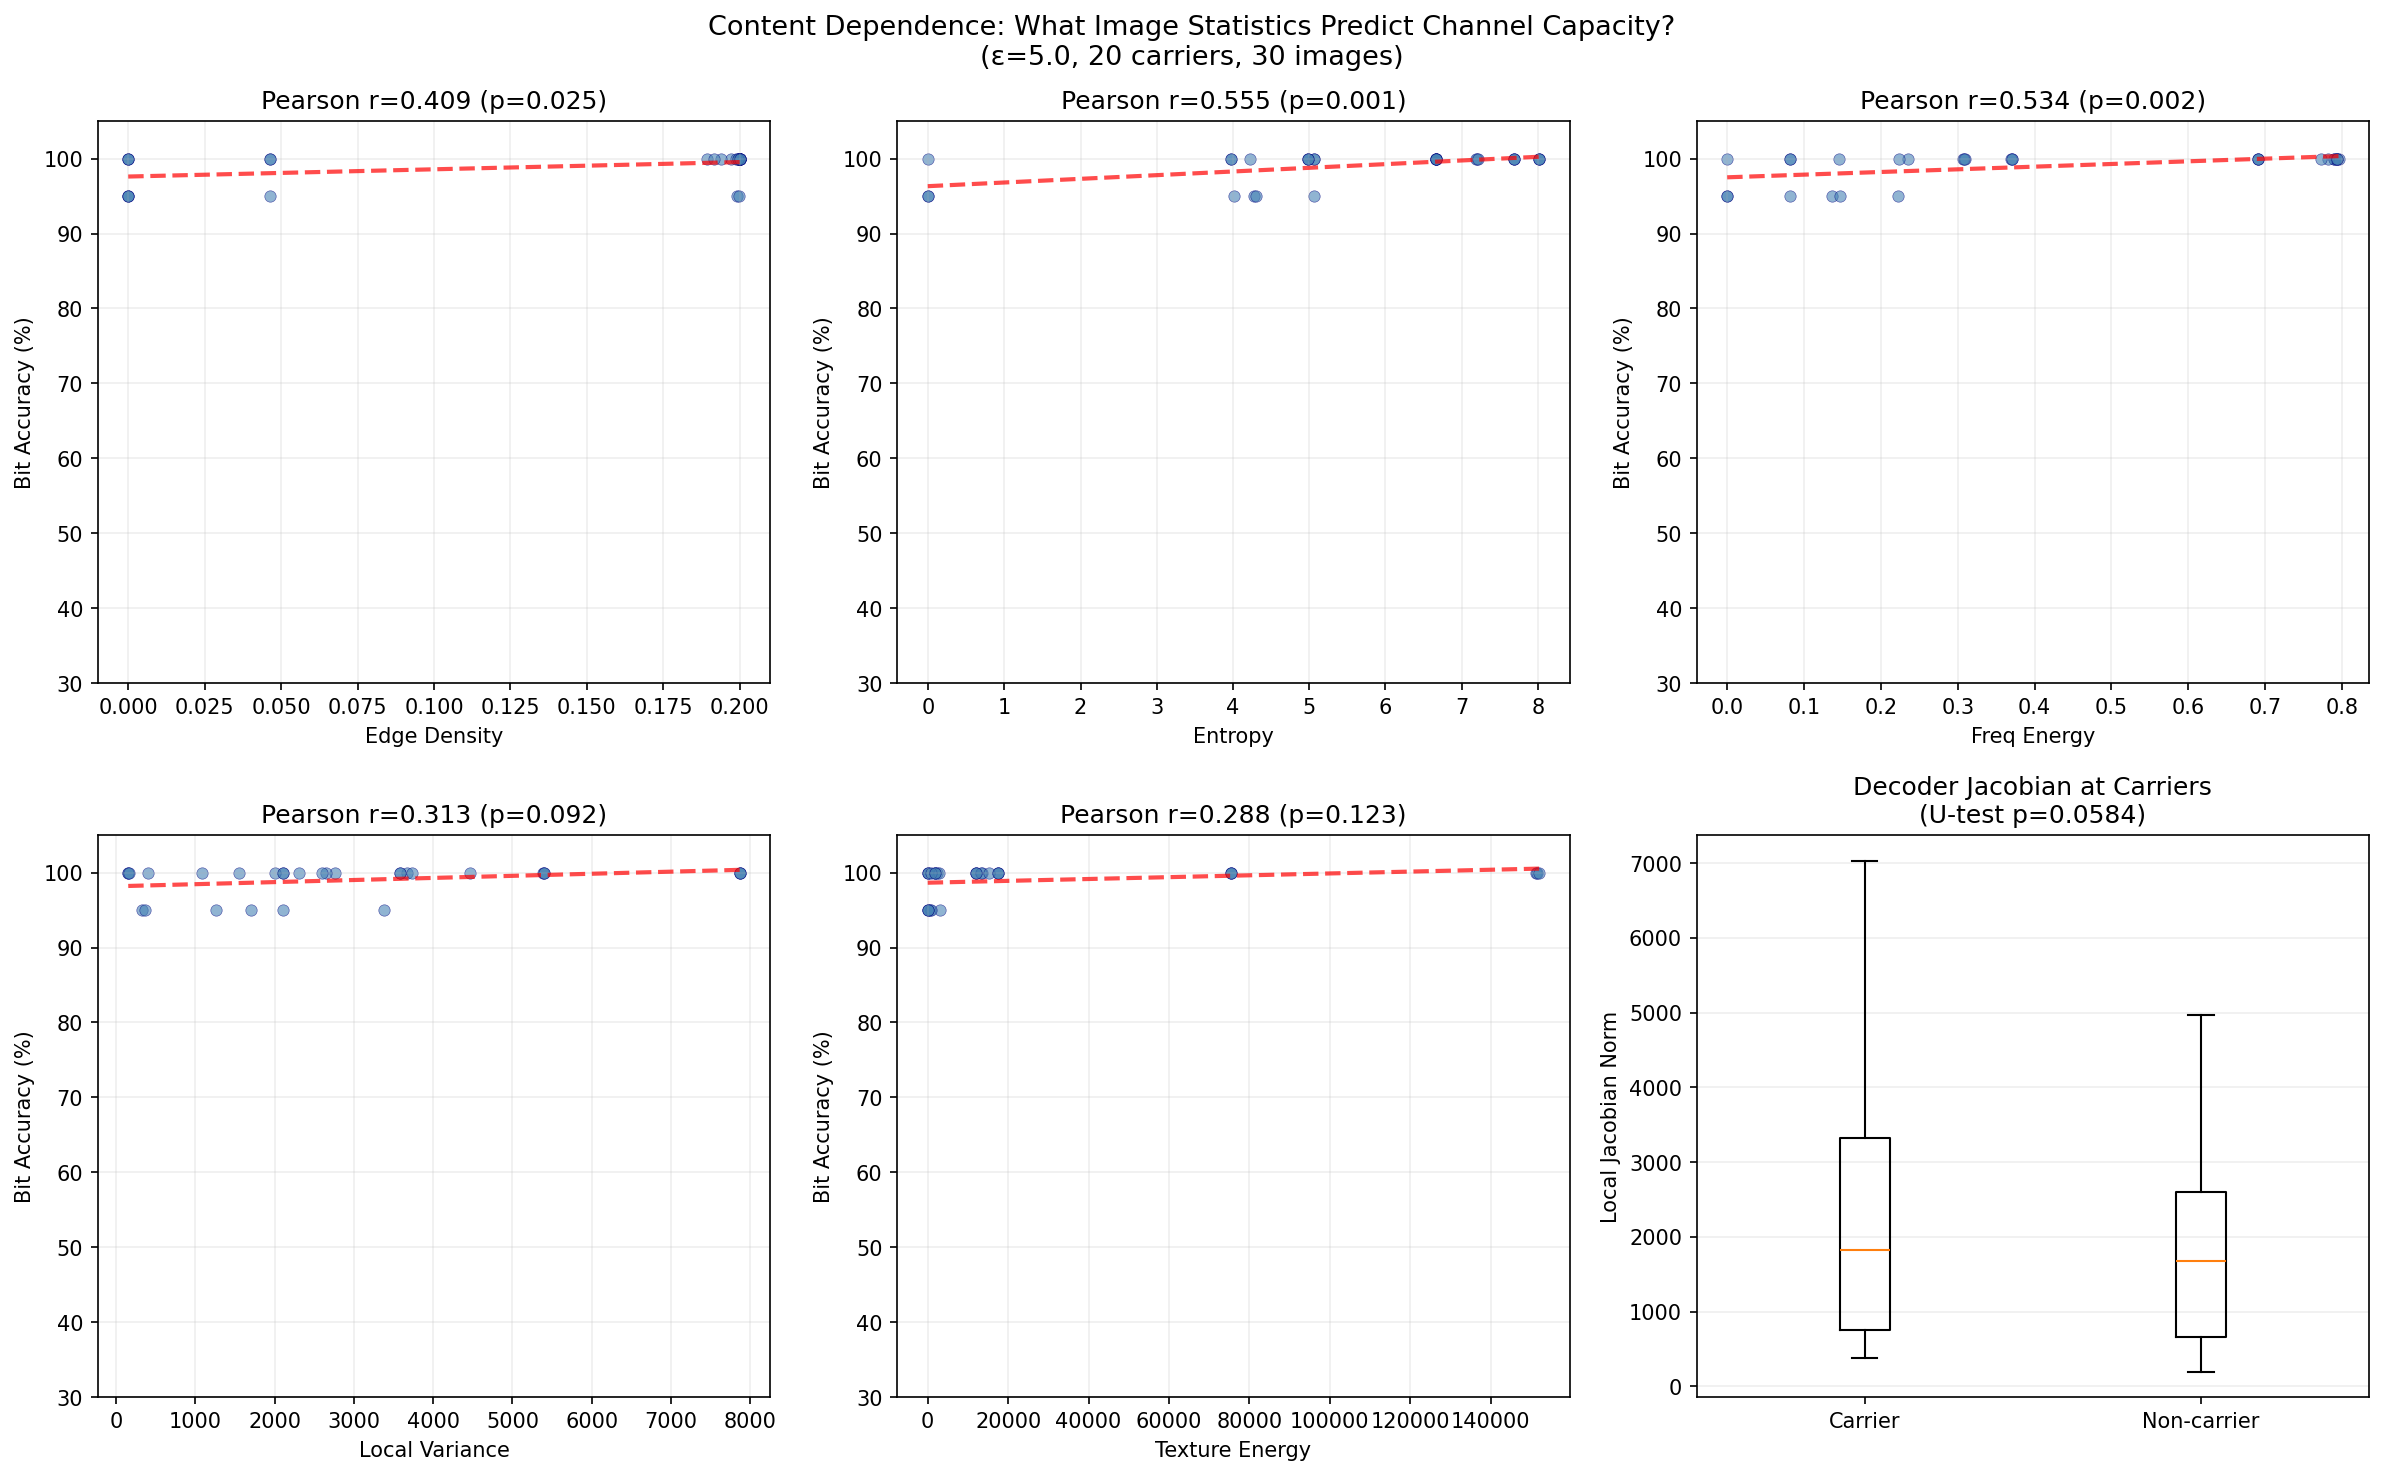
\includegraphics[width=\columnwidth]{../figures/content_science.png}
\caption{Content-dependent diagnostics. Image statistics correlate with bit recovery, and local finite-difference geometry suggests higher sensitivity at selected carriers.}
\label{fig:content}
\end{figure}

\subsection{Natural Images And VAE Backbones}

On 300 CIFAR-10 images, PatchSteg reaches 98.2\% bit accuracy at $\epsilon=2.0$ with 95\% CI [97.8, 98.7], and 98.5\% at $\epsilon=5.0$ with 95\% CI [98.0, 98.9]. Mean PSNR values are 38.6 dB and 28.9 dB. The use of upscaled CIFAR-10 is a limitation; native high-resolution validation is a priority before submission.

\begin{figure}[t]
\centering
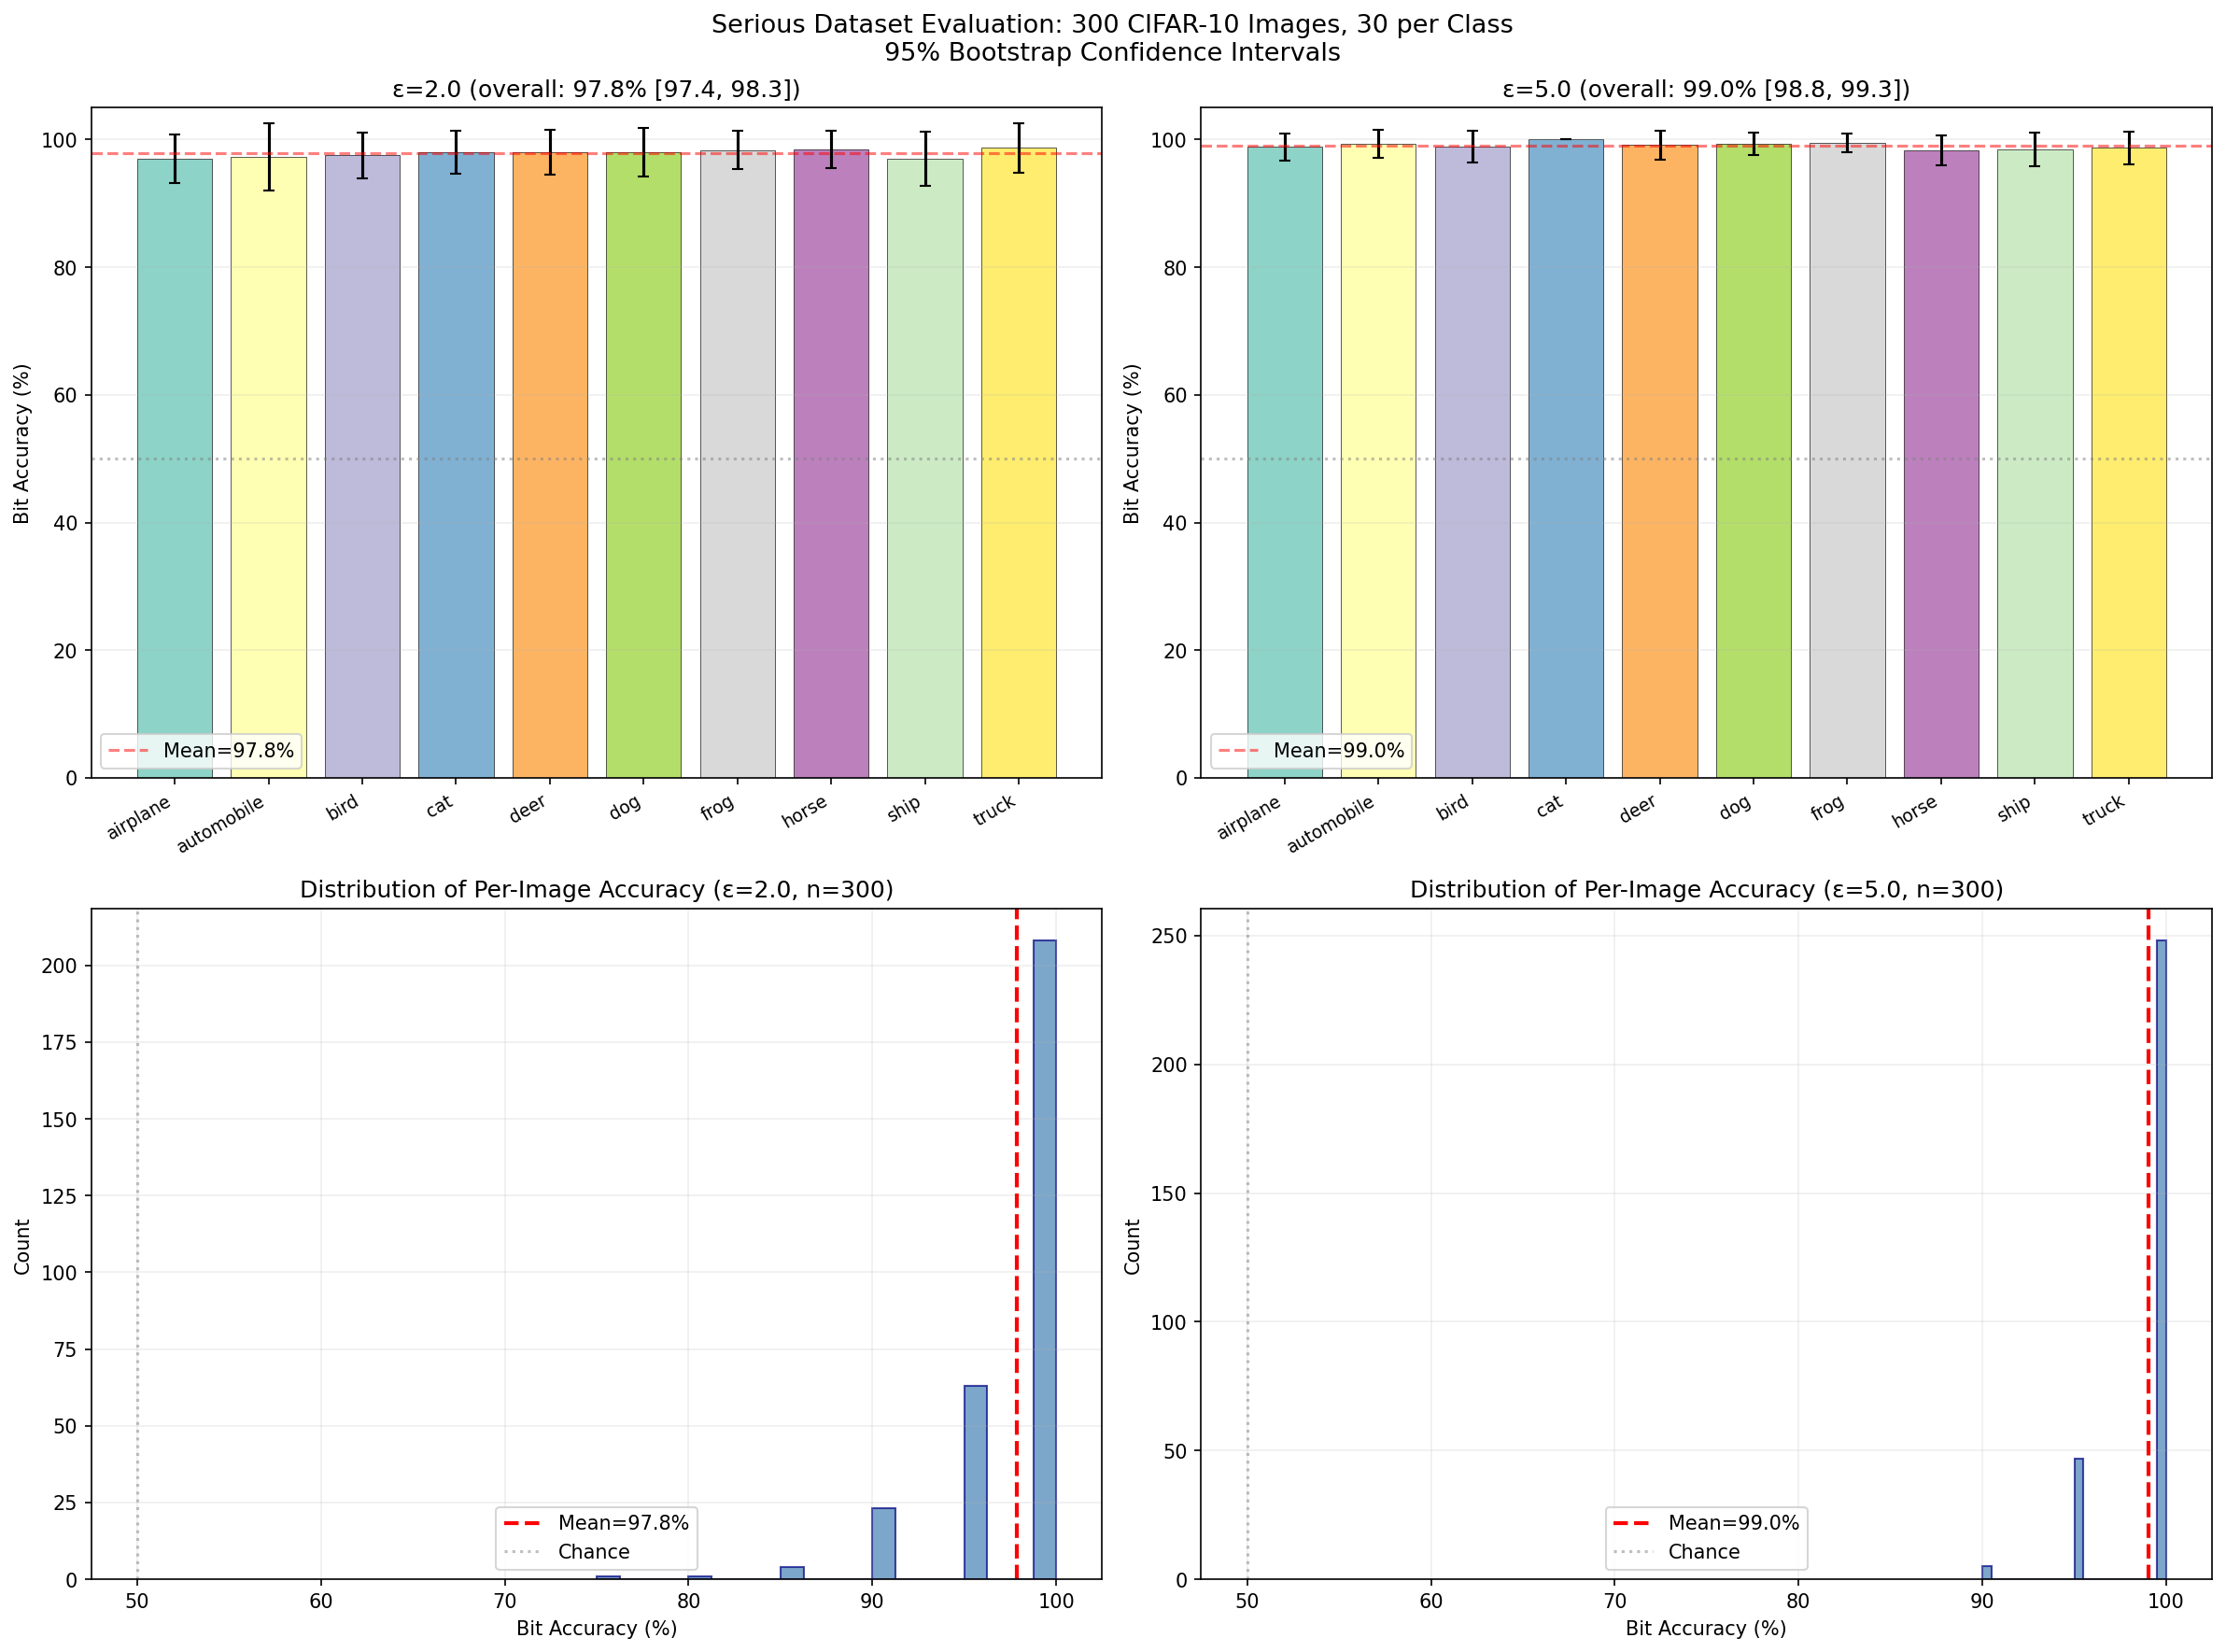
\includegraphics[width=\columnwidth]{../figures/serious_dataset.png}
\caption{Natural-image evaluation on 300 CIFAR-10 images. Recovery remains high across classes, with variation consistent with content-dependent stability.}
\label{fig:natural}
\end{figure}

The effect generalizes across SD-VAE-MSE, SD-VAE-EMA, and SDXL-VAE, with related checkpoints also supporting cross-model decoding.

\begin{figure}[t]
\centering
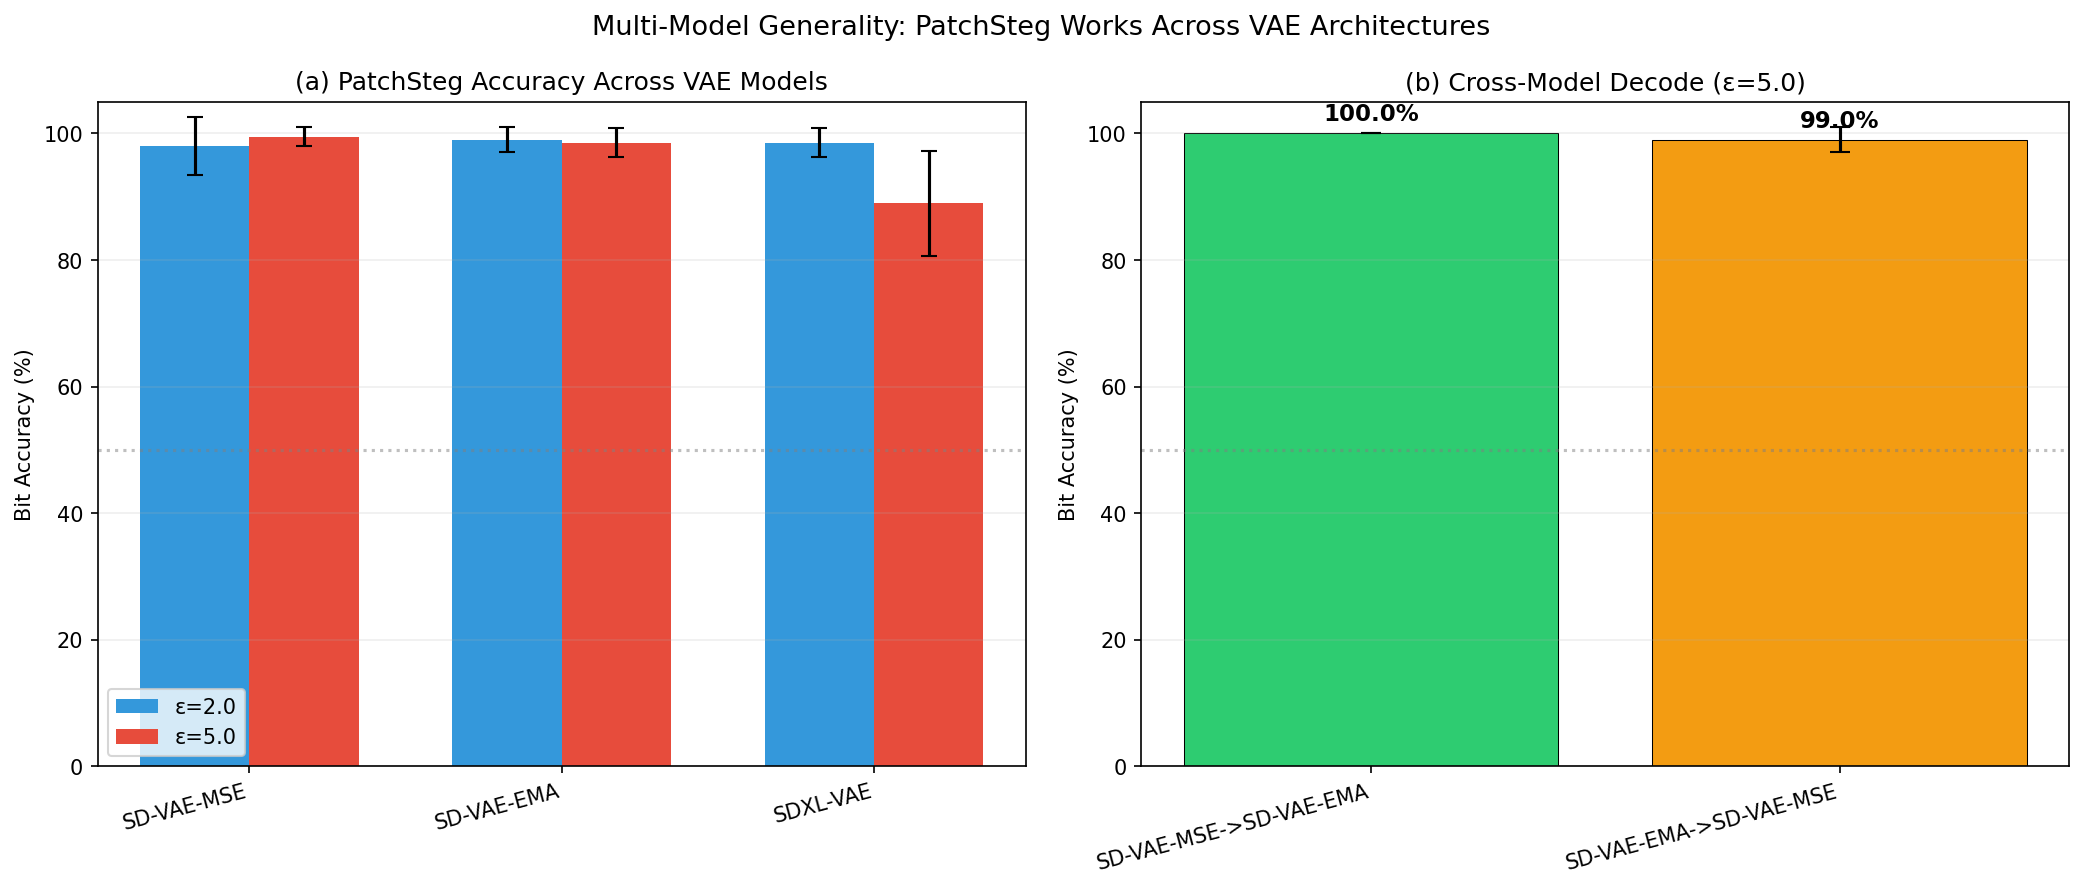
\includegraphics[width=\columnwidth]{../figures/multimodel.png}
\caption{Multi-VAE diagnostic. The failure trigger is not tied to a single model file, though checkpoint choice affects reliability.}
\label{fig:multimodel}
\end{figure}

\subsection{Monitoring Diagnostics}

Increasing $\epsilon$ improves reliability but makes detection easier. A latent-statistics logistic regression detector yields AUC 0.44 at $\epsilon=1.0$, 0.68 at $\epsilon=2.0$, 0.93 at $\epsilon=5.0$, and 0.97 at $\epsilon=10.0$. Stronger detector families can perform better, especially with pixel-residual and spectral features.

\begin{figure}[t]
\centering
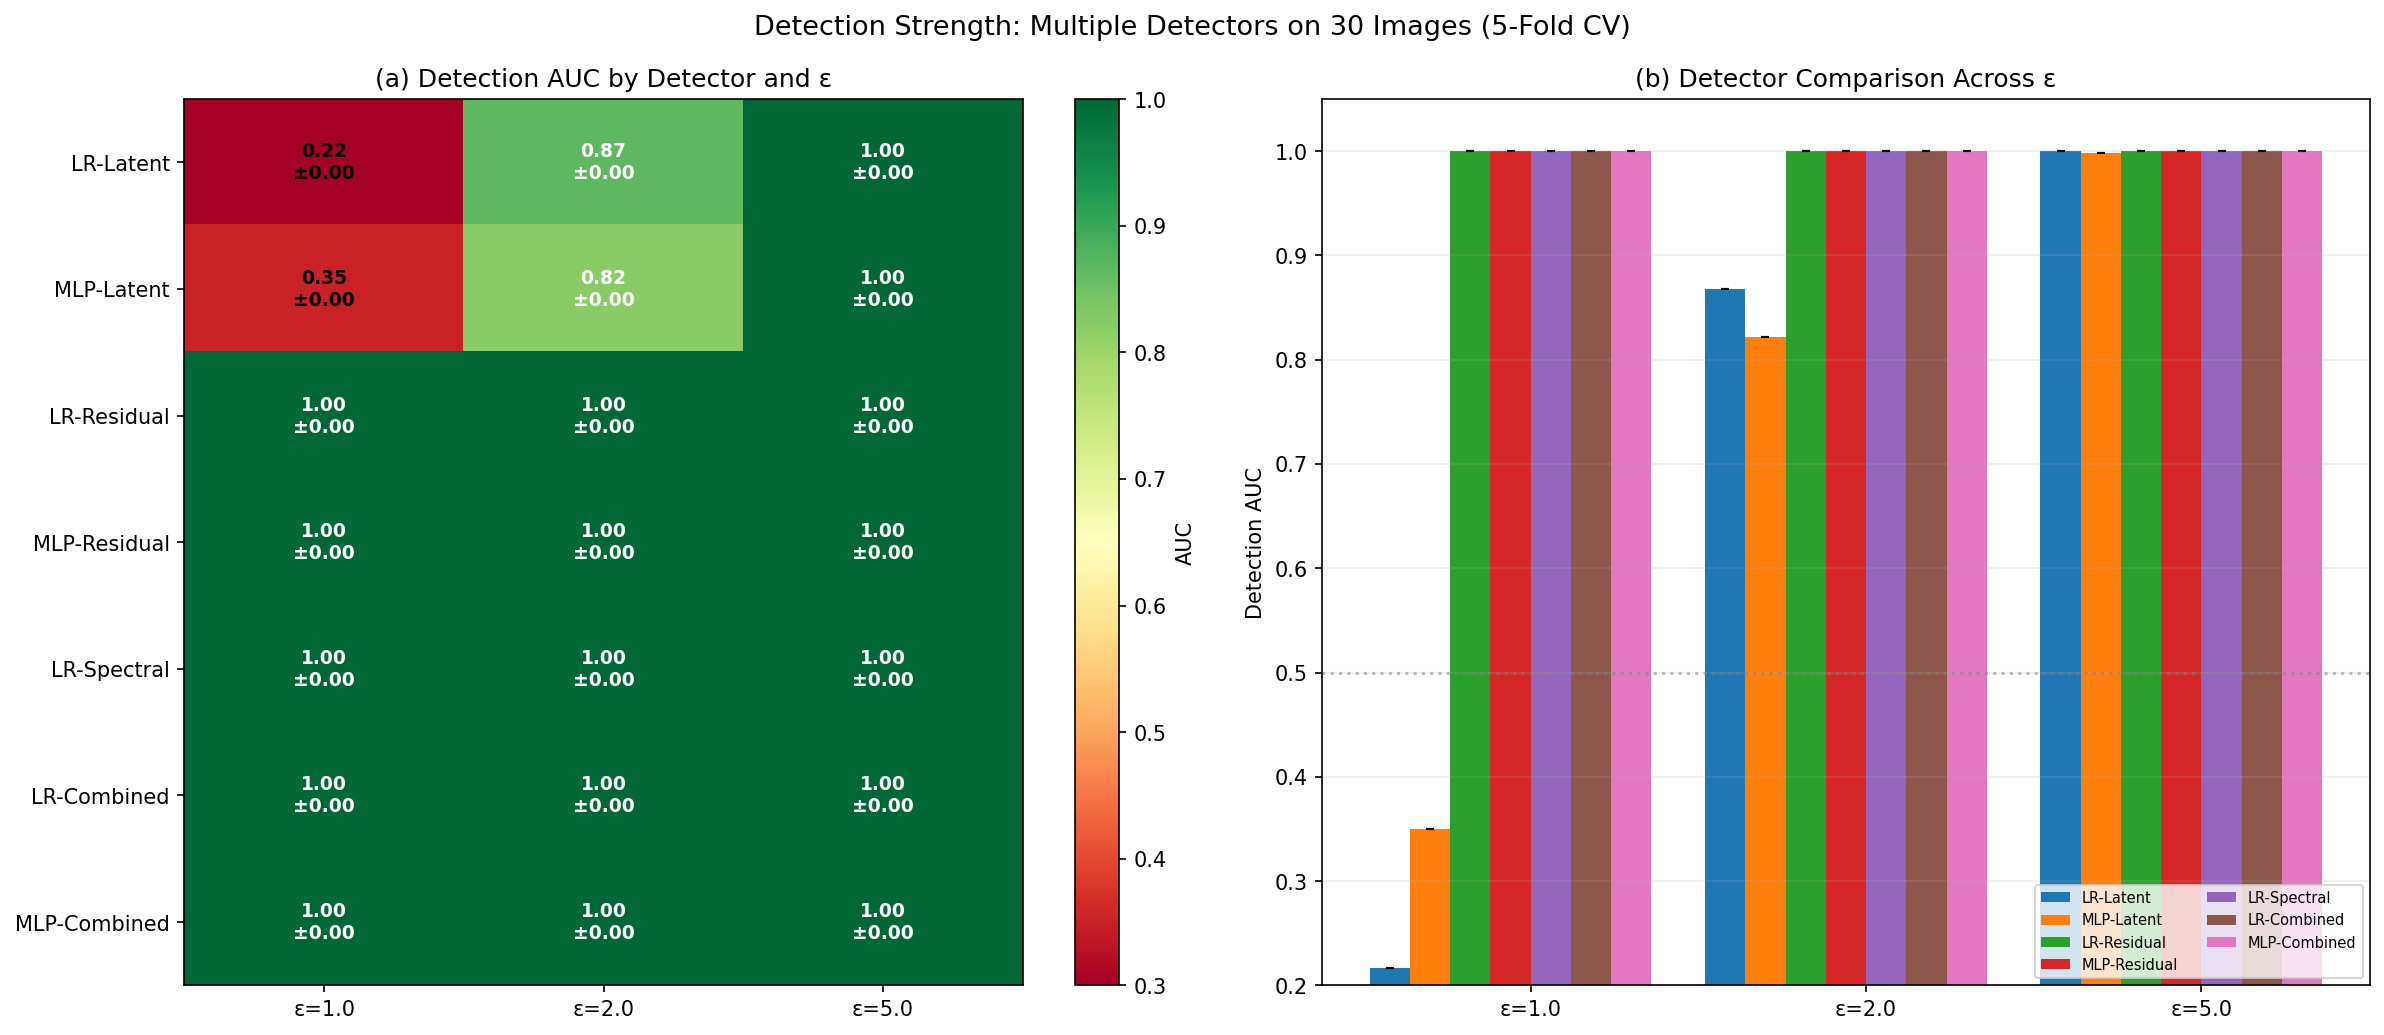
\includegraphics[width=\columnwidth]{../figures/detection_strength.png}
\caption{Detector diagnostics across feature families. The result should be read as a detector-specific monitoring study, not a broad undetectability claim.}
\label{fig:detection}
\end{figure}

\section{Verified Fixes And Negative Results}

We evaluate defenses as partial fixes rather than solved mitigations. Existing sanitizers reduce bit recovery only by paying visible or measurable fidelity costs. The current evidence points to a Pareto tradeoff: aggressive latent smoothing, noise, or quantile reflection disrupts the channel more strongly, but also damages image quality.

\begin{figure}[t]
\centering
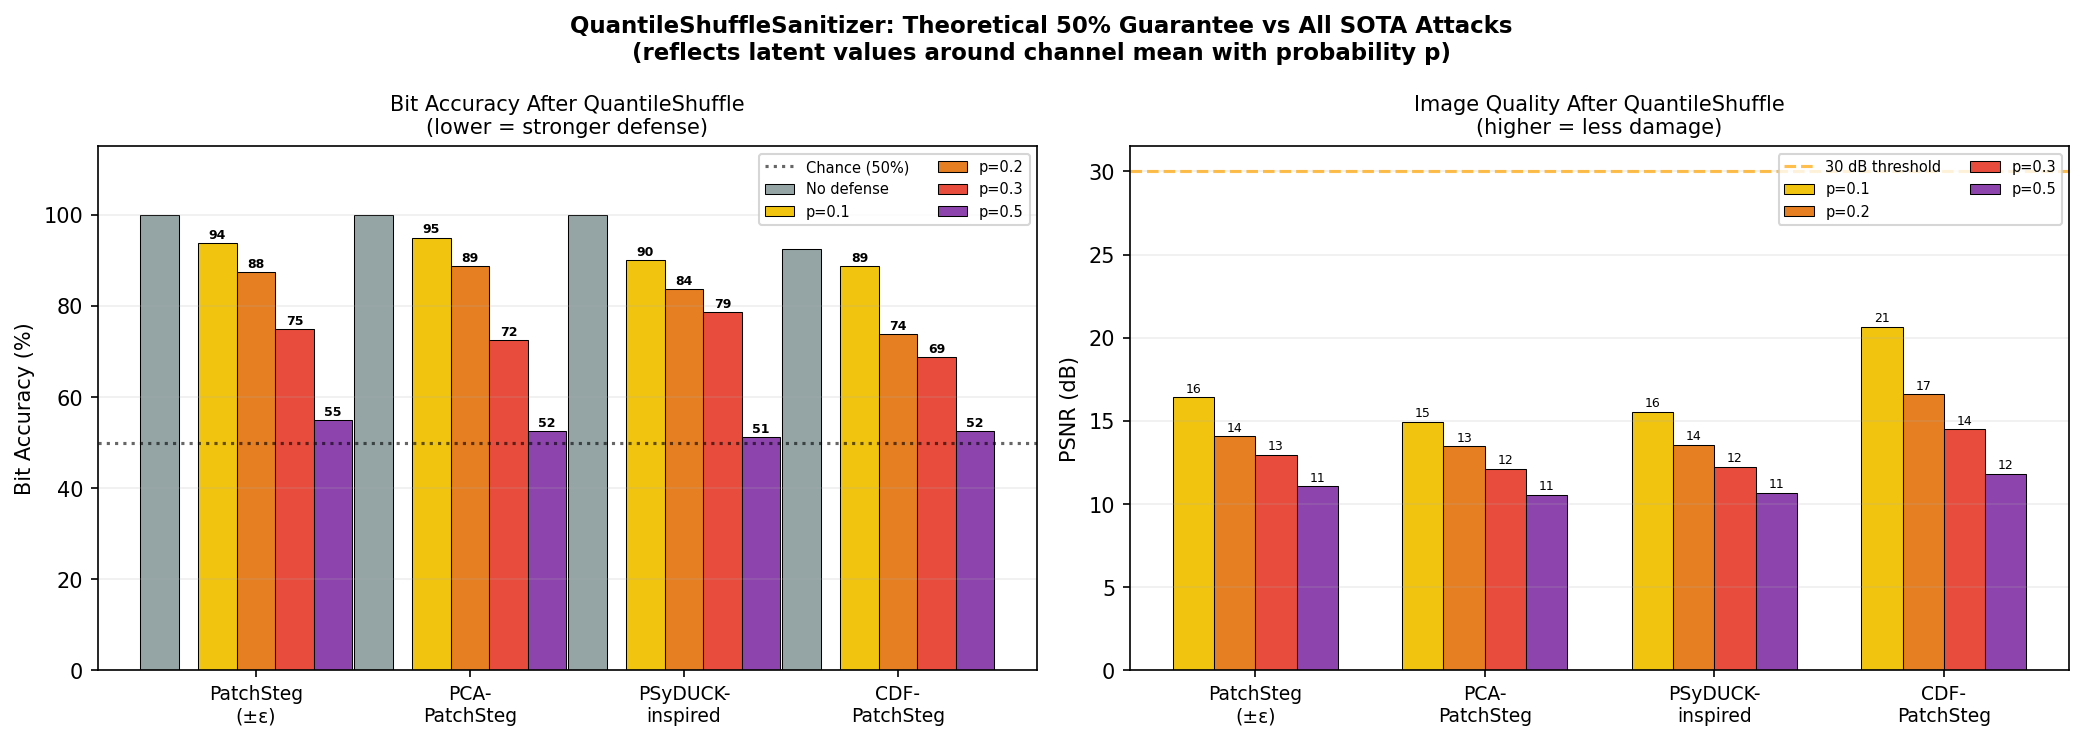
\includegraphics[width=\columnwidth]{../figures/quantile_sanitizer_results.png}
\caption{Sanitizer pilot. Quantile reflection reduces bit accuracy toward chance at high intervention rates, but the fidelity cost is large because many non-carrier positions are modified.}
\label{fig:sanitizer}
\end{figure}

This is a useful negative result for FMAI. Pixel-only monitoring is incomplete; simple detectors are detector-family-specific; and naive sanitization is not free. Before final FMAI submission, the strongest addition would be a full fidelity--disruption Pareto curve over latent smoothing, quantile reflection, additive latent noise, JPEG re-encoding, and low-strength regeneration.

\section{Agent-In-The-Loop Evaluation Plan}

The current paper proves the latent failure trigger but does not yet include a full agent-in-the-loop demonstration. We plan to add a two-agent shared-workspace experiment: a sender embeds a 32-bit payload into a cover image and posts it with an innocuous caption; a receiver extracts the payload; a monitor sees only the image and caption and reports whether anything suspicious is visible. Metrics will include payload recovery rate, monitor flag rate on stego versus clean images, qualitative monitor descriptions, latency, and cost. This experiment is the highest-priority FMAI addition because it connects the VAE-level trigger to deployed agent infrastructure.

\section{Limitations}

PatchSteg assumes a compatible VAE checkpoint, a shared seed, and, for the baseline protocol, a shared clean cover or clean round-trip latent. Most headline natural-image results use upscaled CIFAR-10, so native high-resolution validation is needed. PSNR is incomplete; LPIPS and SSIM should be added to all quality claims. The defense section is currently a pilot and should be replaced by a full sanitizer Pareto. Finally, the mechanistic Jacobian account is suggestive rather than complete.

\section{Conclusion}

PatchSteg is a compact, reproducible failure mode for image-handling agentic AI systems. It provides an operational definition of image-mediated latent covert communication, a simple trigger, interpretable diagnostics, and preliminary fixes whose limitations are measurable. This makes it a strong test case for studying how multimodal agent infrastructure can fail even when visible image content appears benign.

\bibliography{../main}
\bibliographystyle{../../icml2026/icml2026}

\clearpage
\appendix

\section{Appendix Index}

\begin{table*}[t]
\caption{Supplementary material included in the appendix. These figures are retained from the full internal draft for review context; small-n attack and defense variants are exploratory unless explicitly labeled otherwise in the main paper.}
\label{tab:appendix_index}
\centering
\begin{small}
\begin{tabular}{lll}
\toprule
Appendix & Artifact & Purpose \\
\midrule
\ref{app:diagnostics} & Deployment robustness & Shows which image transformations preserve carrier alignment. \\
\ref{app:diagnostics} & Detector ROC curves & Gives additional monitoring diagnostics beyond the main detector figure. \\
\ref{app:diagnostics} & Anomaly-detector heatmap & Records exploratory detector/attack pilot results. \\
\ref{app:variants} & CDF distribution matching & Documents a pilot blind-decoding variant. \\
\ref{app:variants} & PCA direction pilot & Documents data-aligned perturbation directions. \\
\bottomrule
\end{tabular}
\end{small}
\end{table*}

\clearpage
\section{Additional Diagnostics}
\label{app:diagnostics}

\begin{figure*}[t]
\centering
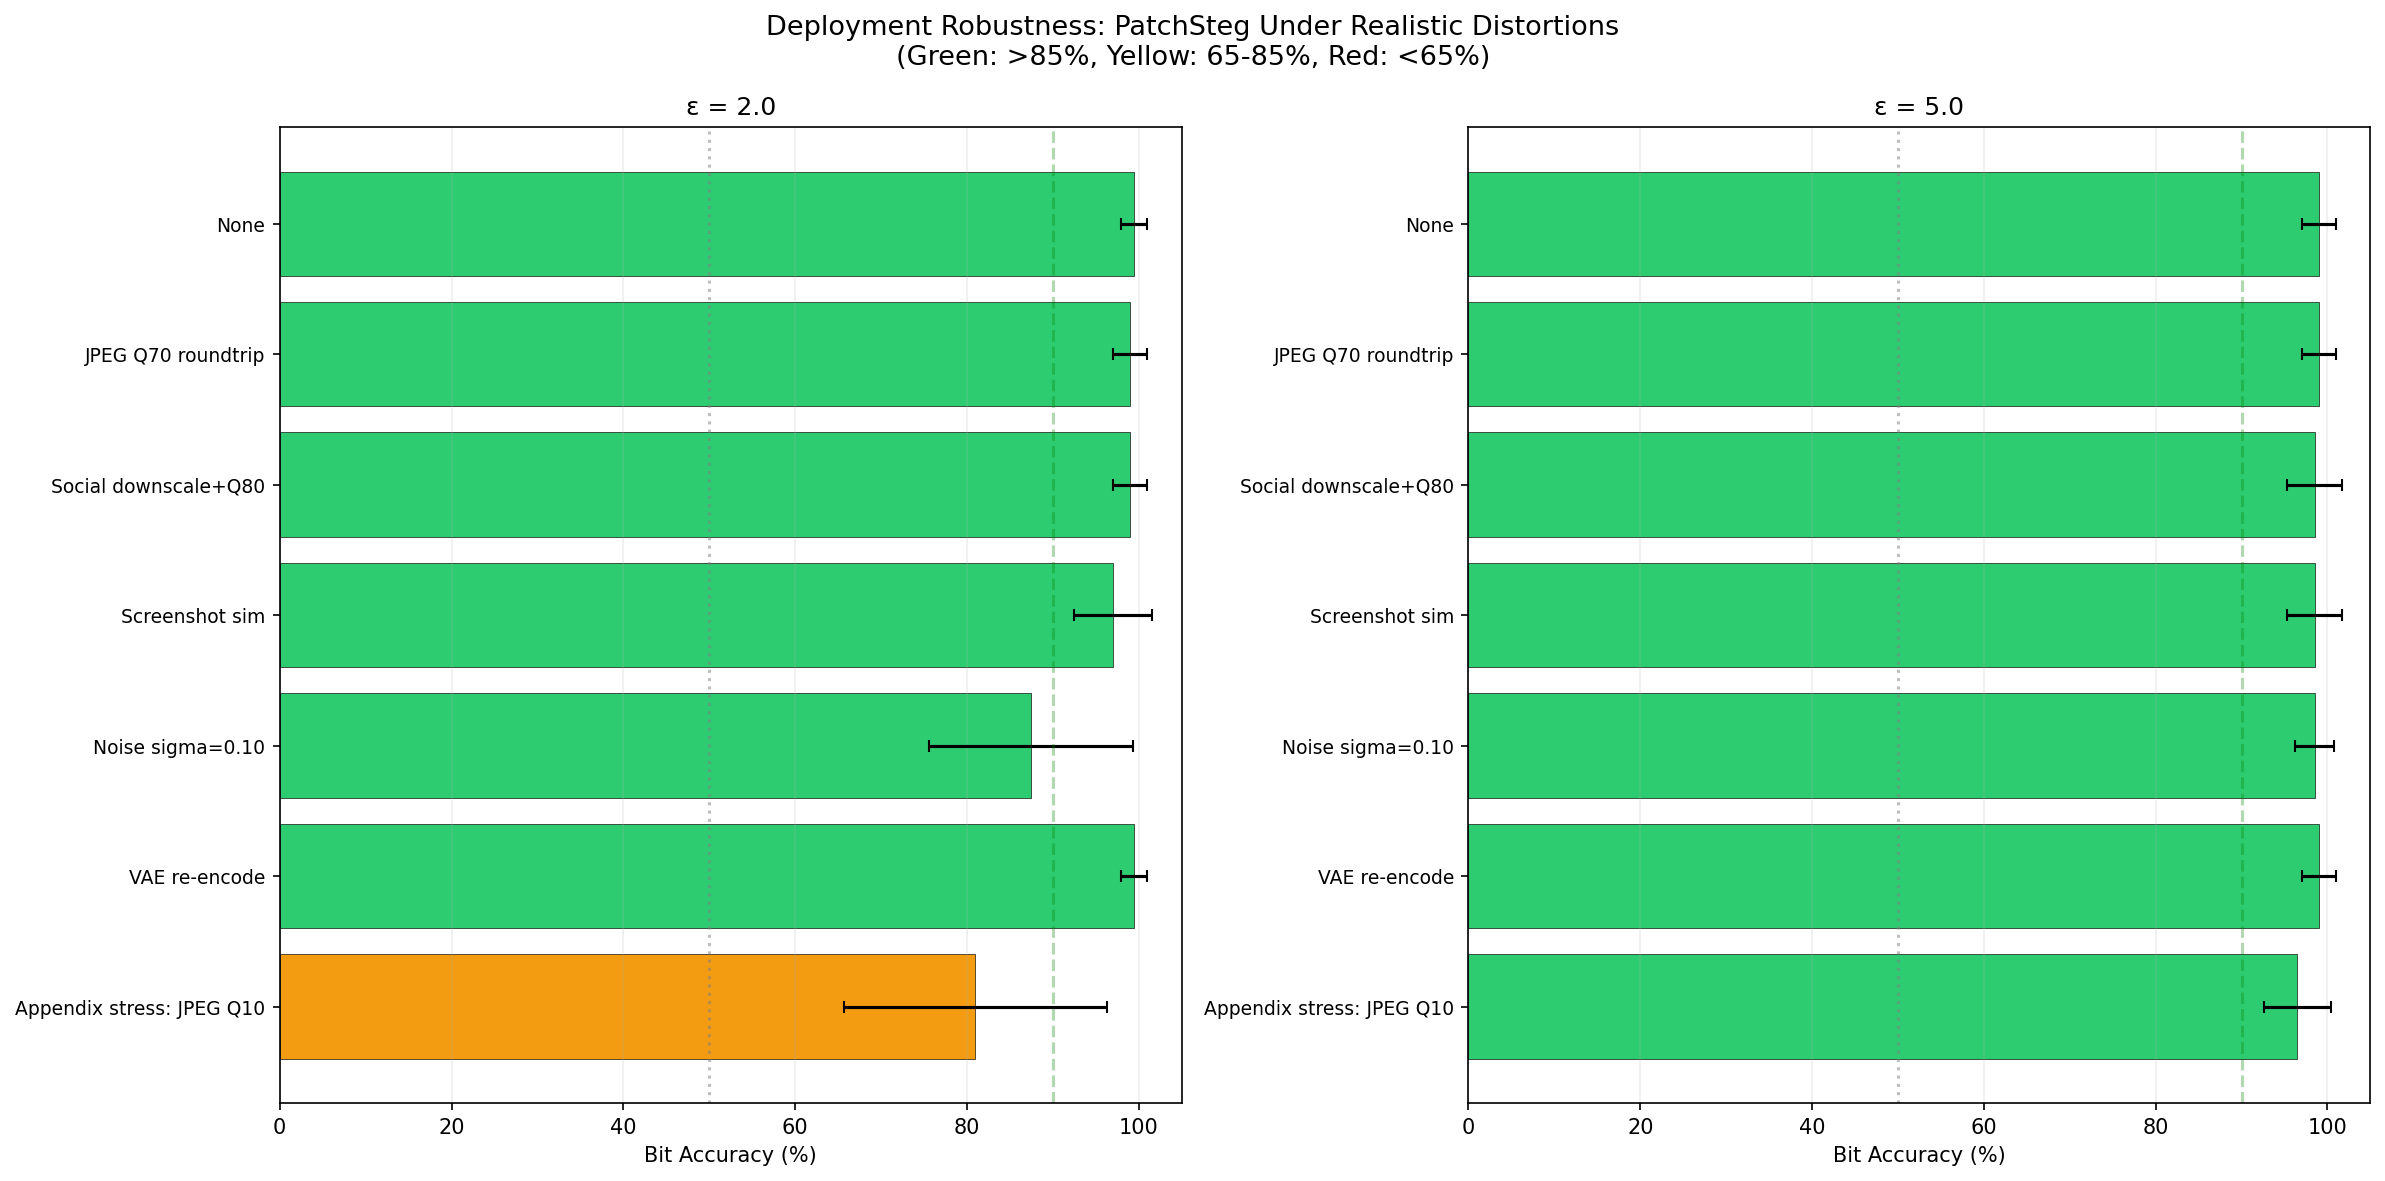
\includegraphics[width=0.82\textwidth]{../figures/deployment_robustness.png}
\caption{Deployment-style robustness diagnostics. Cropping is destructive because it breaks spatial carrier alignment; VAE re-encoding and screenshot simulation preserve high recovery in the current experiment.}
\end{figure*}

\begin{figure*}[t]
\centering

\includegraphics[width=0.82\textwidth]{../figures/detector_roc_curves.png}
\caption{ROC curves for the stronger latent steganalysis detector used in pilot experiments.}
\end{figure*}

\begin{figure*}[t]
\centering
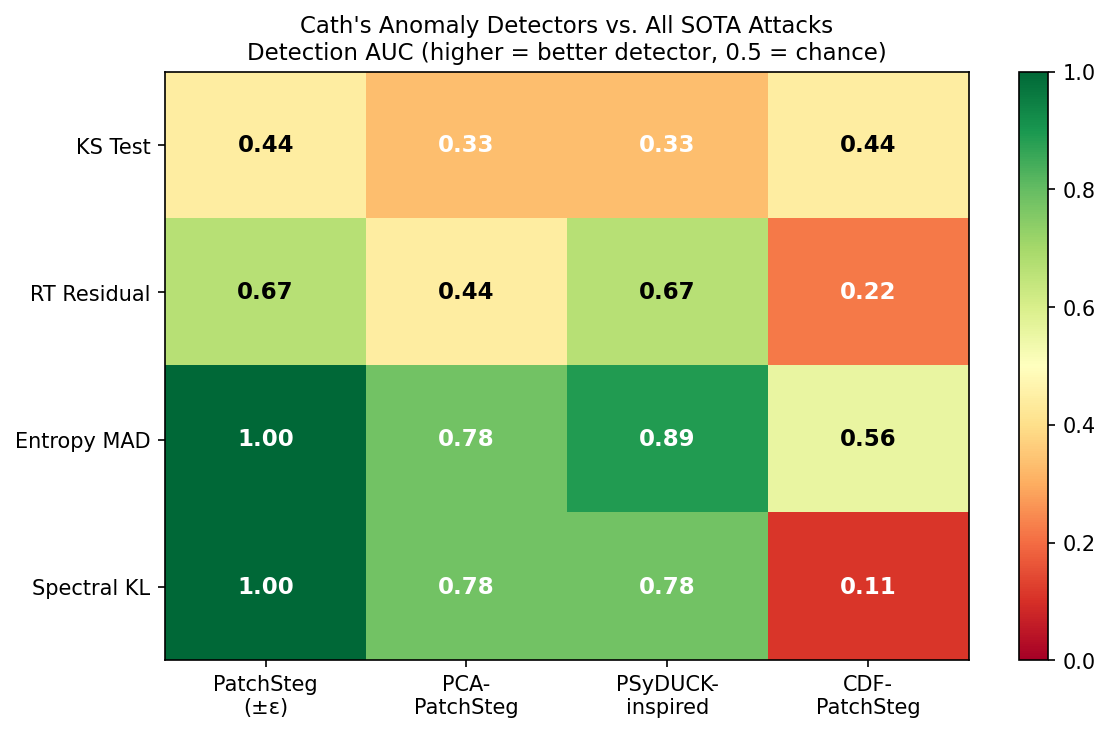
\includegraphics[width=0.72\textwidth]{../figures/cath_defense_heatmap.png}
\caption{Pilot anomaly-detector heatmap across evaluated attack variants. These small-n results should be treated as exploratory.}
\end{figure*}

\clearpage
\section{Exploratory Attack Variants}
\label{app:variants}

\begin{figure*}[t]
\centering

\includegraphics[width=0.82\textwidth]{../figures/cdf_distribution.png}
\caption{CDF-PatchSteg pilot distribution matching. This variant is useful for future safety work but is not central to the FMAI main claim without scaled evaluation.}
\end{figure*}

\begin{figure*}[t]
\centering

\includegraphics[width=0.72\textwidth]{../figures/pca_accuracy_comparison.png}
\caption{PCA-guided direction pilot. Data-aligned directions provide an additional diagnostic of latent geometry.}
\end{figure*}

\end{document}
